%\title{Using the forest package to create trees in LaTeX}
% From http://tex.stackexchange.com/a/108728/23931 
\documentclass[preview,border=0]{standalone}
% \documentclass{article}
\usepackage[paperheight=20cm,paperwidth=13.5cm]{geometry}
\usepackage{graphicx}
% \usepackage{forest}
\usepackage{amsmath}
\usepackage{tikz-qtree}
\usepackage{kmath,kerkis}

\begin{document}
% \vspace*{\fill}
 \begin{center}

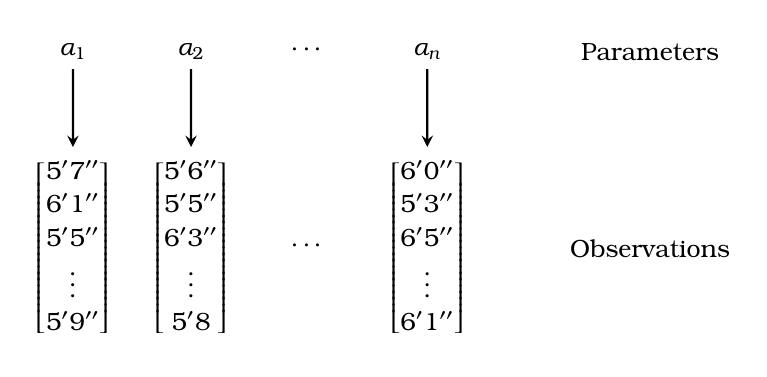
\begin{tikzpicture}[
    thick, % line style
    > = stealth, % arrow head style
    level distance=1.8cm,
    level 1/.style ={level distance=.2cm},
    level 2/.style ={level distance=2.5cm},
    % level 2/.style={sibling distance=1cm},
    % level 3/.style={sibling distance=1cm}
]
% \tikzstyle{every edge}=[circle,draw]
\node (R) {  }
    child {node (a) {$\alpha_1$} 
        child {
            node (b) { $\begin{bmatrix} 5'7'' \\ 6'1'' \\  5'5'' \\ \vdots \\ 5'9'' \end{bmatrix}$ }  
            edge from parent[->] }
        edge from parent[draw=none] 
    }
    child {node {$\alpha_2$} 
        child {
             node { $\begin{bmatrix} 5'6'' \\ 5'5'' \\  6'3'' \\ \vdots \\ 5'8 \end{bmatrix}$ } 
            edge from parent[->] }
        edge from parent[draw=none] 
    }
    child {node {$\cdots$} 
        child {node {$\cdots$} edge from parent[draw=none] }
        edge from parent[draw=none] 
    }
    child {node {$\alpha_n$} 
        child {
            node { $\begin{bmatrix} 6'0'' \\ 5'3'' \\  6'5'' \\ \vdots \\ 6'1'' \end{bmatrix}$ } 
            edge from parent[->] }
        edge from parent[draw=none]
    };

    \path (R) ++(1.5in,0)coordinate(R0)  node [thick] { } ++(.5in,0)  node [] { };
    \node at (a -| R0)(a0) { } (a0)++(.5in,0)  node [] {Parameters};
    \node at (b -| R0)(b0) { } (b0)++(.5in,0)  node [] {Observations};
\end{tikzpicture}


\end{center}
% \vspace*{\fill}
\end{document}
